%%%%%%%%%%%%%%%%%%%%%%%%%%%%%%%%%%%%%%%%%%%%%%%
%
% Template per Elaborato di Laurea
% DISI - Dipartimento di Ingegneria e Scienza dell’Informazione
%
% update 2015-09-10
%
%%%%%%%%%%%%%%%%%%%%%%%%%%%%%%%%%%%%%%%%%%%%%%%

\documentclass[epsfig,a4paper,11pt,titlepage,twoside,openany]{book}

\usepackage{epsfig}
\usepackage{plain}
\usepackage{setspace}
\usepackage{graphicx}
%\usepackage[utf8x]{inputenc} % create conflicts with hyperref
\usepackage{multirow}
\usepackage[table]{xcolor}
\usepackage[paperheight=29.7cm,paperwidth=21cm,outer=1.5cm,inner=2.5cm,top=2cm,bottom=2cm]{geometry}
\usepackage{titlesec}
\usepackage{url}
\usepackage[acronym,section]{glossaries}
\usepackage[american]{babel}
\usepackage{hyperref}
\usepackage{cleveref}
\usepackage{soul}
\usepackage{booktabs}
\usepackage{tabularx} 
\usepackage[ruled,vlined,linesnumbered,resetcount,algochapter]{algorithm2e}
\Crefname{algocf}{Algorithm}{Algorithms}

\definecolor{cloud}{rgb}{0.92, 0.94, 0.95}		% cloud gray
%\input{latex/newCommands}

\singlespacing

\makeglossaries
%% Tutorial on glossaries: https://www.overleaf.com/learn/latex/Glossaries

\newacronym{disi}{DISI}{Department of Information Engineering and Computer Science}
\newacronym{tls}{TLS}{Transport Layer Security}
\newacronym{ac}{AC}{Access Control}
\newacronym{nist}{NIST}{National Institute of Standards and Technology}
\newacronym{us}{US}{United States}
\newacronym{iot}{IoT}{Internet of Things}




\chapter*{Glossary}
\setglossarystyle{altlist}
\printglossaries

\begin{document}
    
    \pagenumbering{gobble} 
    \pagestyle{plain}

\thispagestyle{empty}

\begin{center}
  \begin{figure}[h!]
    \centerline{
\psfig{file=./resources/pdf/unitn.pdf,width=0.6\textwidth}}
  \end{figure}

  \vspace{2 cm} 

  \LARGE{Department of Information Engineering and Computer Science\\}

  \vspace{1 cm} 
  \Large{Master degree in Computer Science - Cyber Security}

  \vspace{2 cm} 
  \Large\textsc{FINAL REPORT\\} 
  \vspace{1 cm} 
  \Huge\textsc{IoT MALWARE: MIRAI\\}

  \vspace{2 cm} 
  \begin{centering}
        \Large{\textbf{Group 4}}\\
        \Large{Luigi Dell'Eva, Riccardo Germenia, Ion Andy Ditu}
  \end{centering}
  \vspace{4 cm} 

  \Large{Academic year 2023/2024}
  
\end{center}
    \clearpage
    \cleardoublepage
    
    \pagestyle{plain}
    
    \mainmatter
    
    \tableofcontents
    
    \begingroup
        %\renewcommand{\cleardoublepage}{} 
        %\renewcommand{\clearpage}{} 
        \titleformat{\chapter}{\normalfont\Huge\bfseries}{\thechapter}{1em}{}
        \titlespacing*{\chapter}{0pt}{0.59in}{0.02in}
        \titlespacing*{\section}{0pt}{0.20in}{0.02in}
        \titlespacing*{\subsection}{0pt}{0.10in}{0.02in}
        \newpage
        %% Tutorial on glossaries: https://www.overleaf.com/learn/latex/Glossaries

\newacronym{disi}{DISI}{Department of Information Engineering and Computer Science}
\newacronym{tls}{TLS}{Transport Layer Security}
\newacronym{ac}{AC}{Access Control}
\newacronym{nist}{NIST}{National Institute of Standards and Technology}
\newacronym{us}{US}{United States}
\newacronym{iot}{IoT}{Internet of Things}




\chapter*{Glossary}
\setglossarystyle{altlist}
\printglossaries
        \newpage
                
        \glsresetall
        
        \chapter{Introduction}
\label{chapter:introduction}

\section{DDoS}

\section{Botnet}

A botnet is a network of internet-connected devices, such as computers, smartphones or IoT devices, whose security has been compromised and control has been taken over by a third party. Botnets were initially designed for legitimate purposes, such as automating repetitive tasks or managing chatroom. However, their ability to execute code within other computers led to their misuse for malicious activities, such as stealing passwords, tracking user keystrokes, and launching attacks against unsuspecting devices. \cite{fortinet-botnet} They are one of the most common types of \textbf{network-based attacks} today due to their use of large, coordinated groups of hosts. These groups are created by infecting vulnerable hosts,  turning them into ``\textit{zombies}'' or \textbf{bots}, which can then be controlled remotely. When a collection of bots is managed by a \textbf{Command and Control} (CNC) infrastructure, it forms a botnet. Botnets help in obscuring the identity of the attacking host by providing a layer of indirection, separating the attacking host from its victim through zombie hosts, and separating the attack itself from the botnet assembly by an arbitrary amount of time. \cite{strayer2008botnet} The method of controlling bots varies based on the architecture of the botnet's command and control mechanisms, which can be \textbf{Internet Relay Chat} (IRC), \textbf{HTTP}, \textbf{DNS}, or \textbf{P2P-based}. 

\section{Mirai}

Mirai is a malware that targets \textbf{IoT devices}, such as routers, cameras and others, by exploiting their default credentials. Once a device is compromised by Mirai, it becomes part of a botnet that can be used to launch \textbf{DDoS attacks}, however, this does not compromise the device's functionality except for occasional increased bandwidth usage. It is capable of running on various CPU architectures, including MIPS, ARM, and others. It uses a dictionary attack with a set of 62 entries to gain control of vulnerable devices. The infected devices are reported to a control server to become part of a large-scale Agent-Handler botnet. \cite{de2018ddos}

The botnet was first created by a guy named Paras Jha, who used it to launch multiple DDoS attacks against Minecraft servers. This was to extort money from the server owners, who would pay him to gain ``protection'' from the attacks. Then it was also used to attack Rutgers University, where he was a student. After these events, he joined forces with other two individuals, Josiah White and Dalton Norman, to further develop the malware, which later became known as Mirai. The malware was first discovered by MalwareMustDie, a non-profit security research group, in August 2016. In the late September of the same year, it gained public attention after being used in a DDoS attack against the Krebs On Security website, reaching 620 Gbps. Following this, it was employed in an attack on the French hosting company OVH, which peaked at 1 Tbps. After these attacks, Anna-senpai, which seems to be the online nickname of Paras Jha, released the source code of Mirai on HackForums\footnote{Original post: \url{https://hackforums.net/showthread.php?tid=5420472}}. This led to the proliferation of Mirai-based botnets and some time later caused the Dyn DDoS attack, which took down several high-profile websites, such as GitHub, Twitter, Reddit, and Netflix. Dyn estimated that up to 100,000 malicious endpoints were involved in the attack. \cite{8115504}

\subsection{Mirai architecture}

The architecture of Mirai is illustrated in \Cref{fig:mirai-architecture} and is based on a \textbf{centralized} model. The botnet is composed of four main components: 

\begin{itemize}
    \item \textbf{CNC server}: the central component of the botnet, it is used by the admin / users to control the bots and to send commands to them.
    \item \textbf{Bots}: the infected devices that are part of the botnet and are used to launch DDoS attacks. Other than waiting for commands to perform attacks, each bot performs some other tasks:
    \begin{itemize}
        \item \textbf{Scanner}: perform active scanning of the internet for vulnerable devices, once found it reports them to the report server. When a device is found it tries to remotely access by using a dictionary based attack with a set of 62 entries. If the attack is successful, the bot will send the vulnerability to the reporting server.
        \item \textbf{Killer}: tries to kill other malware running on the device.
        \item \textbf{Masking}: once the malware is running, it deletes itself from the device to go unnoticed.
    \end{itemize}
    \item \textbf{Reporting server}: its role is to receive the vulnerability (IP, port and potential username and password) found by the bots and forward them to the loader. 
    \item \textbf{Loader server}: it is in charge of loading the malware on the reported devices. 
\end{itemize}

To summarize, Mirai uses a spreading model named ``Real Time Loading'', which is based on the following steps: Bots $\rightarrow$ Reporting server $\rightarrow$ Loader server $\rightarrow$ Bots. \cite{de2018ddos} More information on how the components works with some code snippets can be found in \Cref{chapter:mirai-static-analysis}.


\begin{figure}[ht]
    \centering
    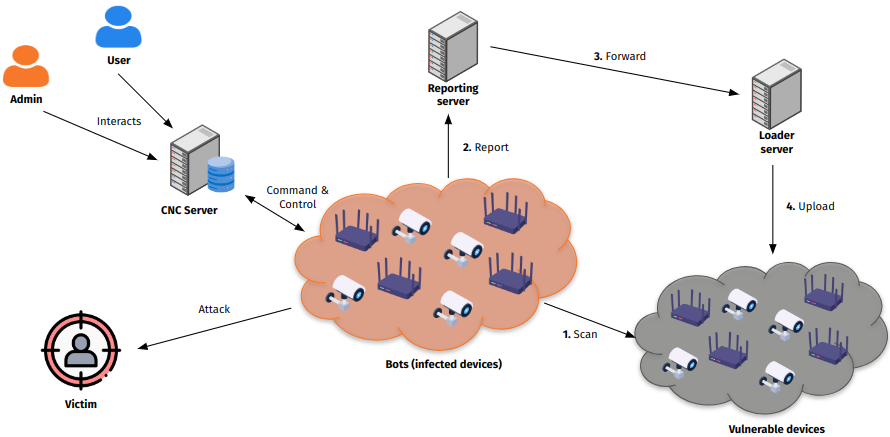
\includegraphics[scale=0.5]{resources/images/mirai-architecture.png}
    \caption{Mirai architecture}
    \label{fig:mirai-architecture}
\end{figure}
        \chapter{Mirai static analysis}
\label{chapter:mirai-static-analysis}

In this chapter we delve into the inner workings of Mirai providing a more technical view over its source code. We will go through some of the most important functions and data structures used by Mirai to infect and control IoT devices.

\section{Directory hierarchy}

The original directory hierarchy of Mirai is shown in \Cref{fig:folder-hierarchy}, and it is composed of the following directories: \texttt{dlr}, \texttt{Loader}, \texttt{Mirai} and \texttt{Scripts}. Note that in our repository this structure can be found into \texttt{unmodified\_code} while in order to make the malware running in our environment we had to make some changes to the original code and its structure. 

\begin{figure}[ht]
    \centering
    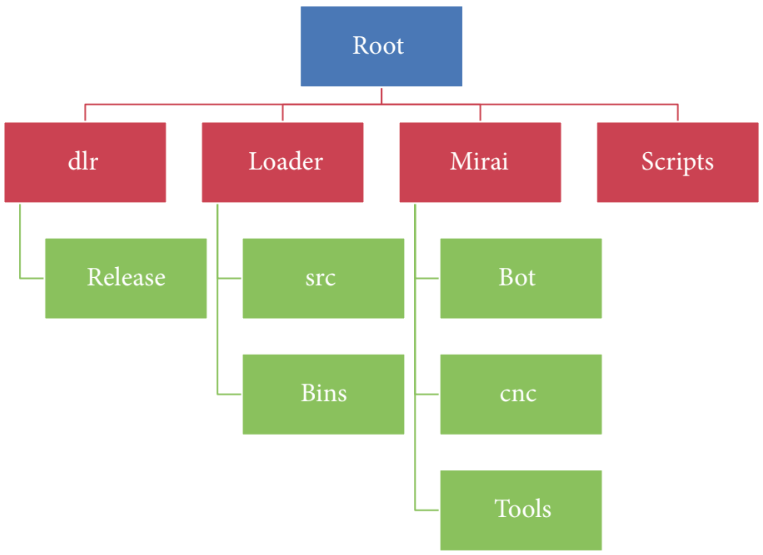
\includegraphics[scale=0.4]{resources/images/folder-structure.png}
    \caption{Original Mirai directory hierarchy \cite{de2018ddos}}
    \label{fig:folder-hierarchy}
\end{figure}

\begin{itemize}
    \item \texttt{dlr}: contains the script needed to compile the \texttt{echoloader} which is a small binary ($\sim$1 KB) that will serve as wget or tftp. The subfolder \texttt{release} contains the echoloader compiled binaries.
    \item \texttt{Loader}: contains the file to execute the loader server. The \texttt{src} subfolder contains its source code and the \texttt{bins} one the binary files of both Mirai malware and the echoloader. 
    \item \texttt{Mirai}: contains the source code of the Mirai malware. This folder is divided into three subfolders:
    \begin{itemize}
        \item \texttt{CNC}: contains the source code of the CNC server written in GO language. 
        \item \texttt{Bot}: contains the source code of the Mirai bots written in C language.
        \item \texttt{Tools}: contains some utility scripts needed to deploy the malware, such as the \texttt{enc.c} script used to encrypt the configuration file and the \texttt{scanListen.go} which implements the Reporting server.
    \end{itemize}
    \item \texttt{Scripts}: contains some utility scripts to compile the malware.
\end{itemize}

Note that the following code snippets are taken from the original Mirai source code, but some part of the code might have been cut out for clarity.

\section{Loader server}

As we said in \Cref{chapter:introduction} the \textbf{Loader server} is in charge of receiving the vulnerabilities from the Reporting server and use them to load the malware on the reported devices. The vulnerabilities received must be in the following format:

\[ \text{\texttt{ip:port} \texttt{user:pass}} \]

The Loader has three main components:
\begin{itemize}
    \item \textbf{Pool of workers}: a worker is a thread whose job is to process the received vulnerabilities and infect the devices. 
    \item \textbf{List of vulnerabilities}: list of information that can be used to access the insecure devices. 
    \item \textbf{Binary source code}: cross-compiled binary for different architectures. 
\end{itemize}

The source code of the loader is into the \texttt{loader/src} folder. The entry point is the \texttt{main.c} file where all the needed data structures are initialized and it has two main parts:

\begin{itemize}
    \item The \texttt{server\_create} function which is illustrated in \Cref{fig:server-create}. It takes as input the \textbf{numbers of workers} to create and both the \textbf{IP address} and \textbf{port} for \textbf{wget} and \textbf{tftp}.
    \item Then it starts \textbf{listening} for incoming reports from the Reporting server. When a report is received, it calls the \texttt{server\_queue\_telnet} function which checks if maximum number of connection (variable \texttt{max\_open}) has been reached. If not, it invokes \texttt{server\_telnet\_probe}. This is shown in \Cref{fig:mainloop}.
\end{itemize}

\begin{figure}[ht]
    \centering
    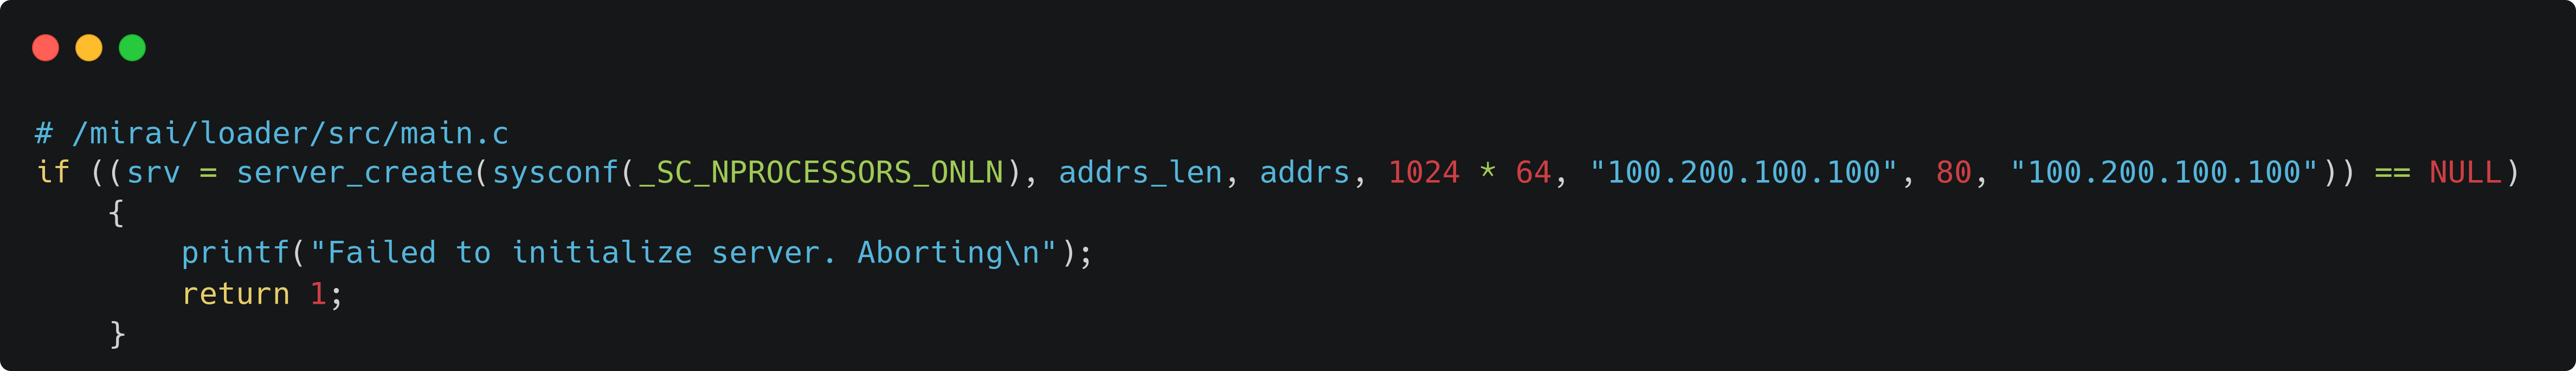
\includegraphics[scale=0.1]{resources/images/server_create.png}
    \caption{\texttt{server\_create} function}
    \label{fig:server-create}
\end{figure}

\begin{figure}[ht]
    \centering
    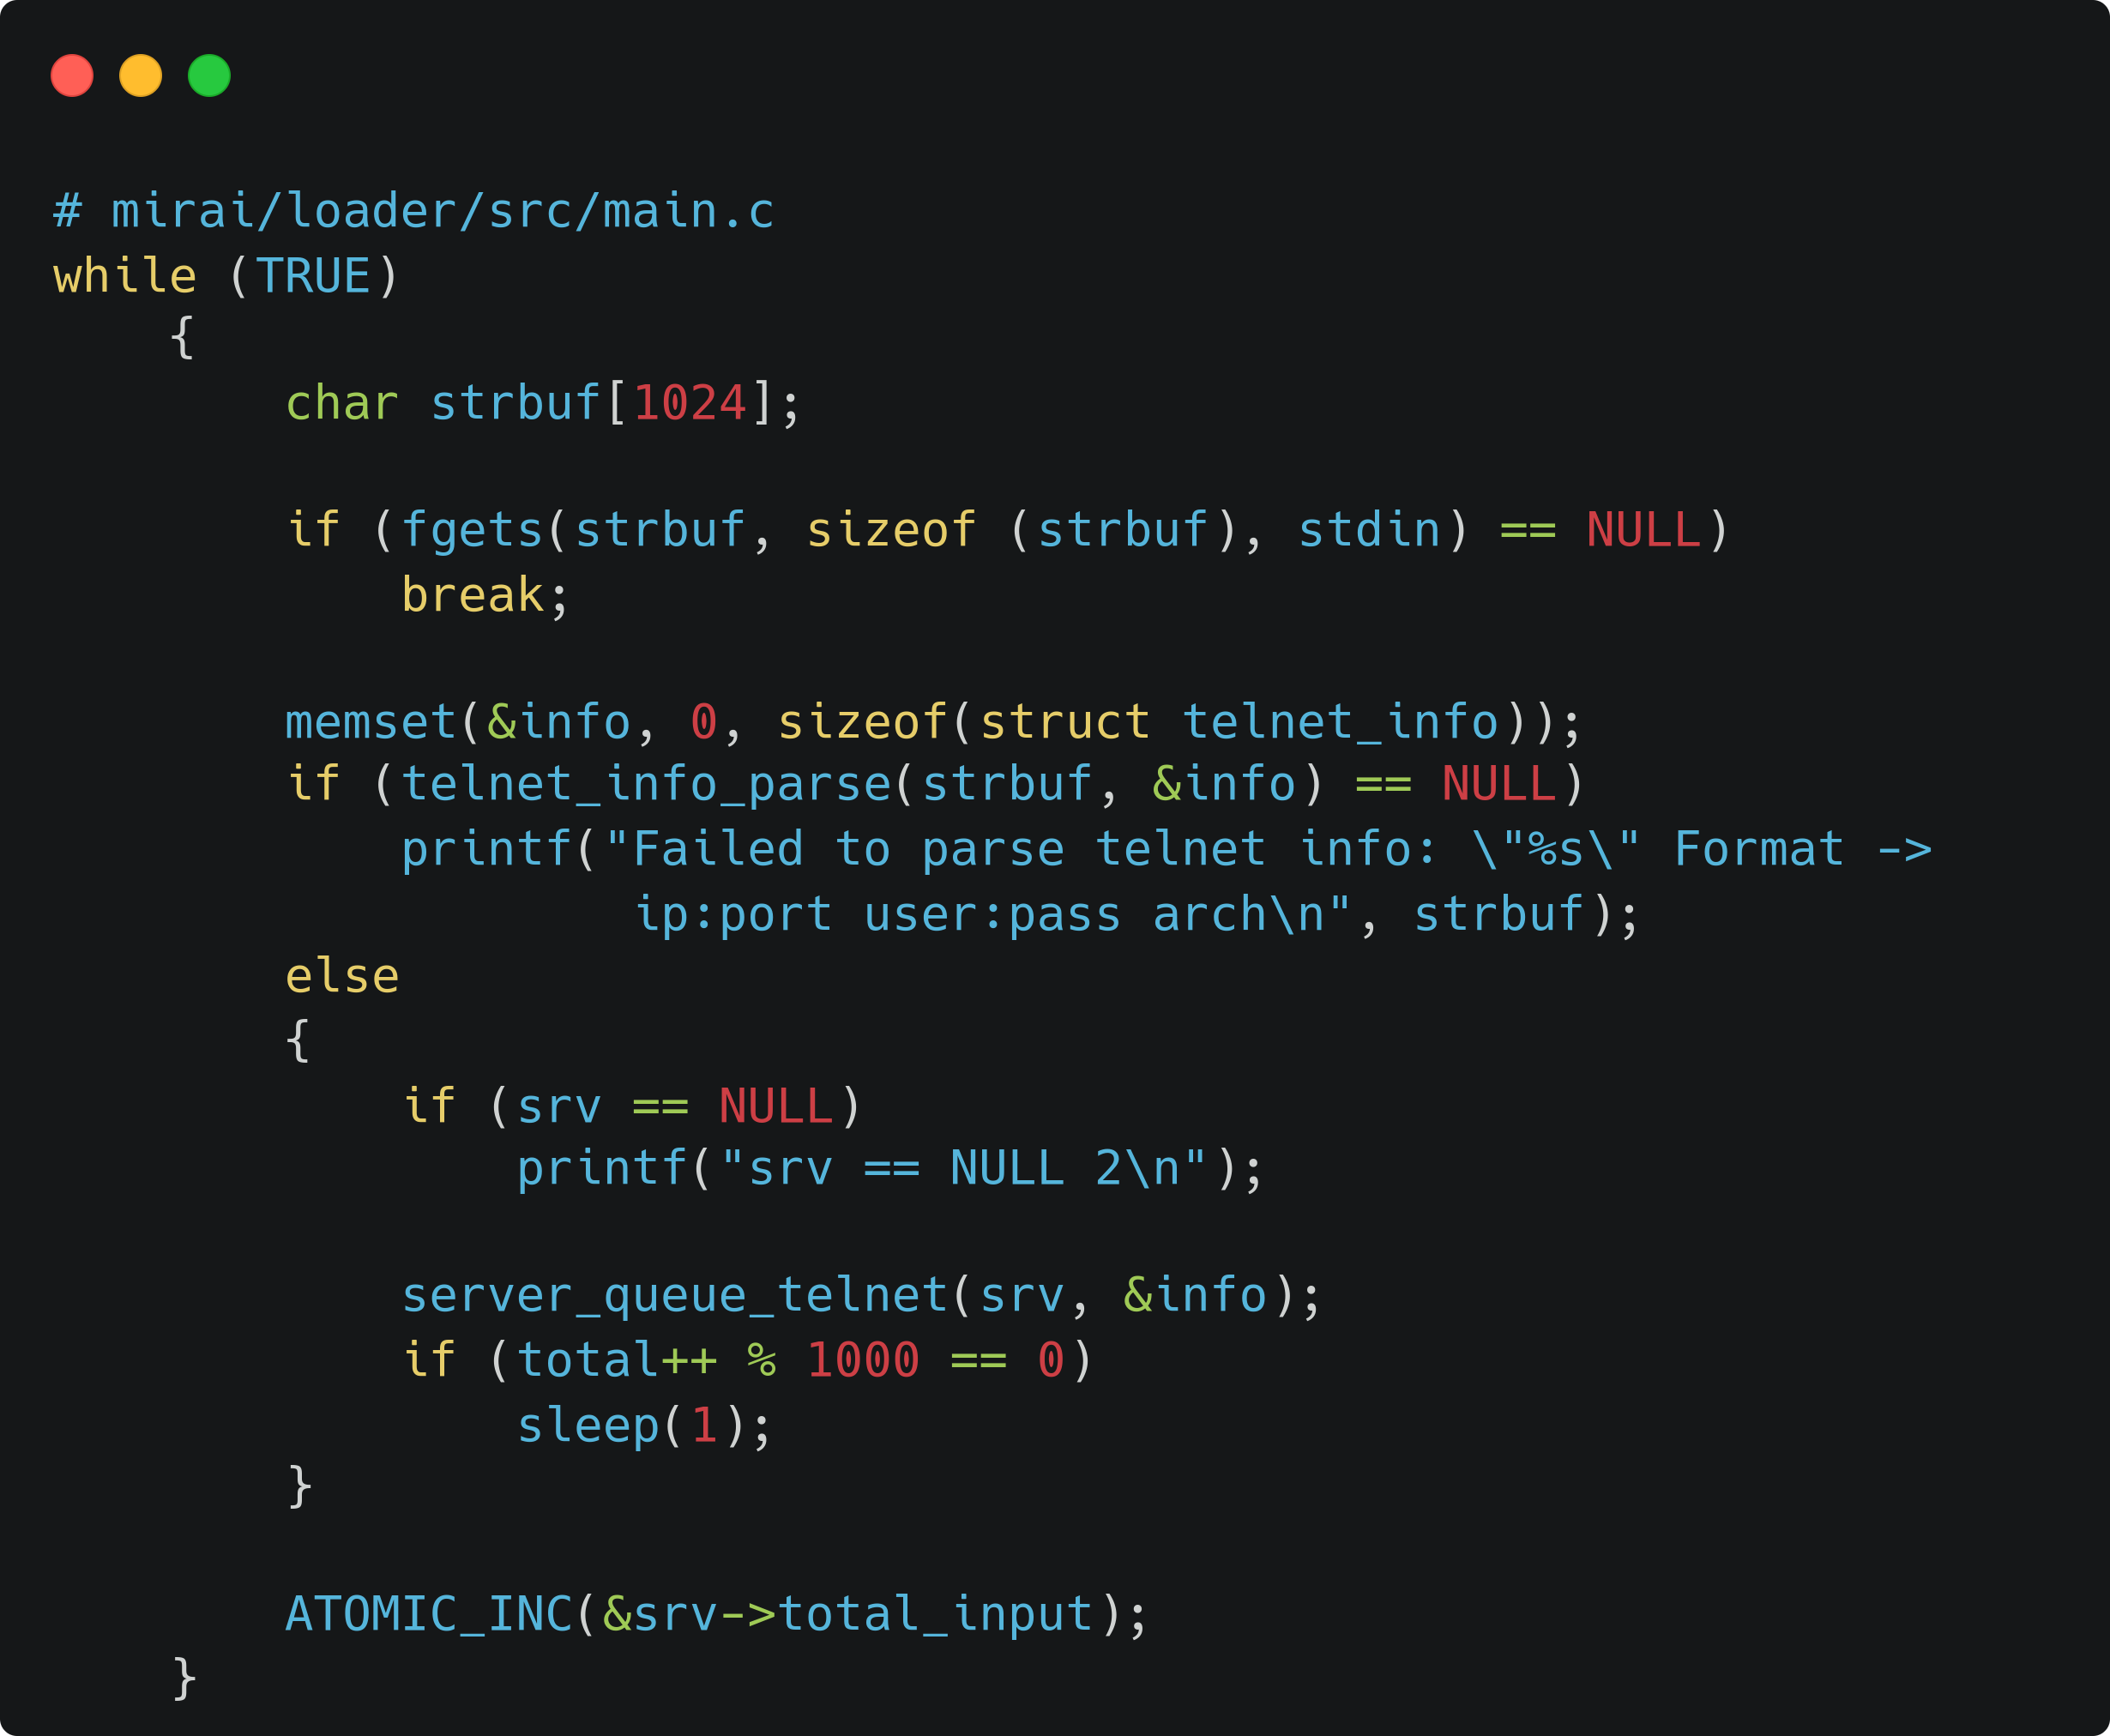
\includegraphics[scale=0.15]{resources/images/main.png}
    \caption{\texttt{main.c} loop}
    \label{fig:mainloop}
\end{figure}

The \texttt{server\_telnet\_probe} is shown in \Cref{fig:server-telnet-probe}. Its role is to \textbf{set up a connection} with the remote device and \textbf{cyclically} add new \textbf{event} to the epoll of the selected worker. In this way as soon as a worker is free, it will be able to call \texttt{handle\_event}.

\begin{figure}[ht]
    \centering
    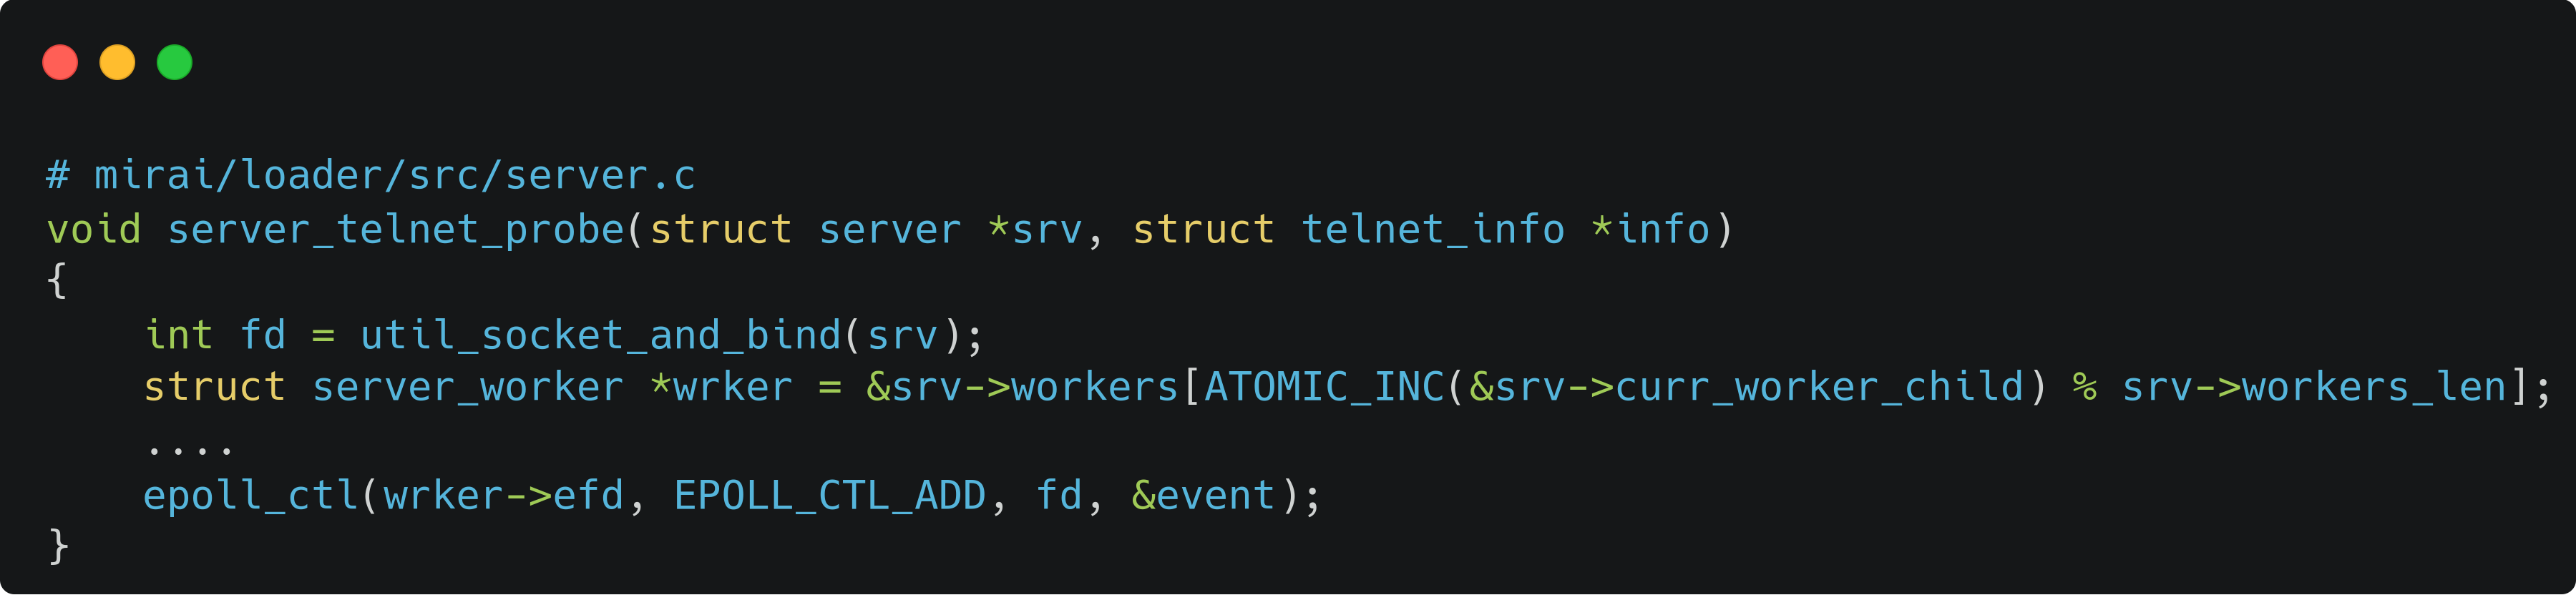
\includegraphics[scale=0.15]{resources/images/sever_telnet_probe.png}
    \caption{\texttt{server\_telnet\_probe} function}
    \label{fig:server-telnet-probe}
\end{figure}

Since the source code of the \texttt{handle\_event} is quite long, we will not show it here. Its role is to interact with the remote device using a switch statement that performs \textbf{various actions} based on a \textbf{state machine}, which is shown in a simplified way in \Cref{fig:state-machine}

\begin{figure}[ht]
    \centering
    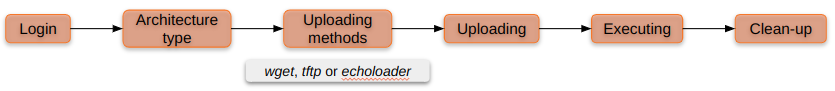
\includegraphics[scale=0.5]{resources/images/state-machine.png}
    \caption{State machine of the \texttt{handle\_event} function}
    \label{fig:state-machine}
\end{figure}

What we have said so far, can be summarized as follow: when a vulnerability result is received, it is added to a worker's list of vulnerabilities. All workers are actively waiting for elements in their lists to process. Once a vulnerability is available, a worker uses the information to access a weak device. It then identifies the device's architecture to load the appropriate executable. The worker tries to upload the binary code to the device using either wget or tftp . If neither is available, the ``echoloader'', which functions similarly to wget, is loaded onto the victim using the Linux echo command and is then used to upload the worm binary code. Once uploaded, it is executed and the device is turned into a Mirai bot.\cite{de2018ddos}

\begin{figure}
    \centering
    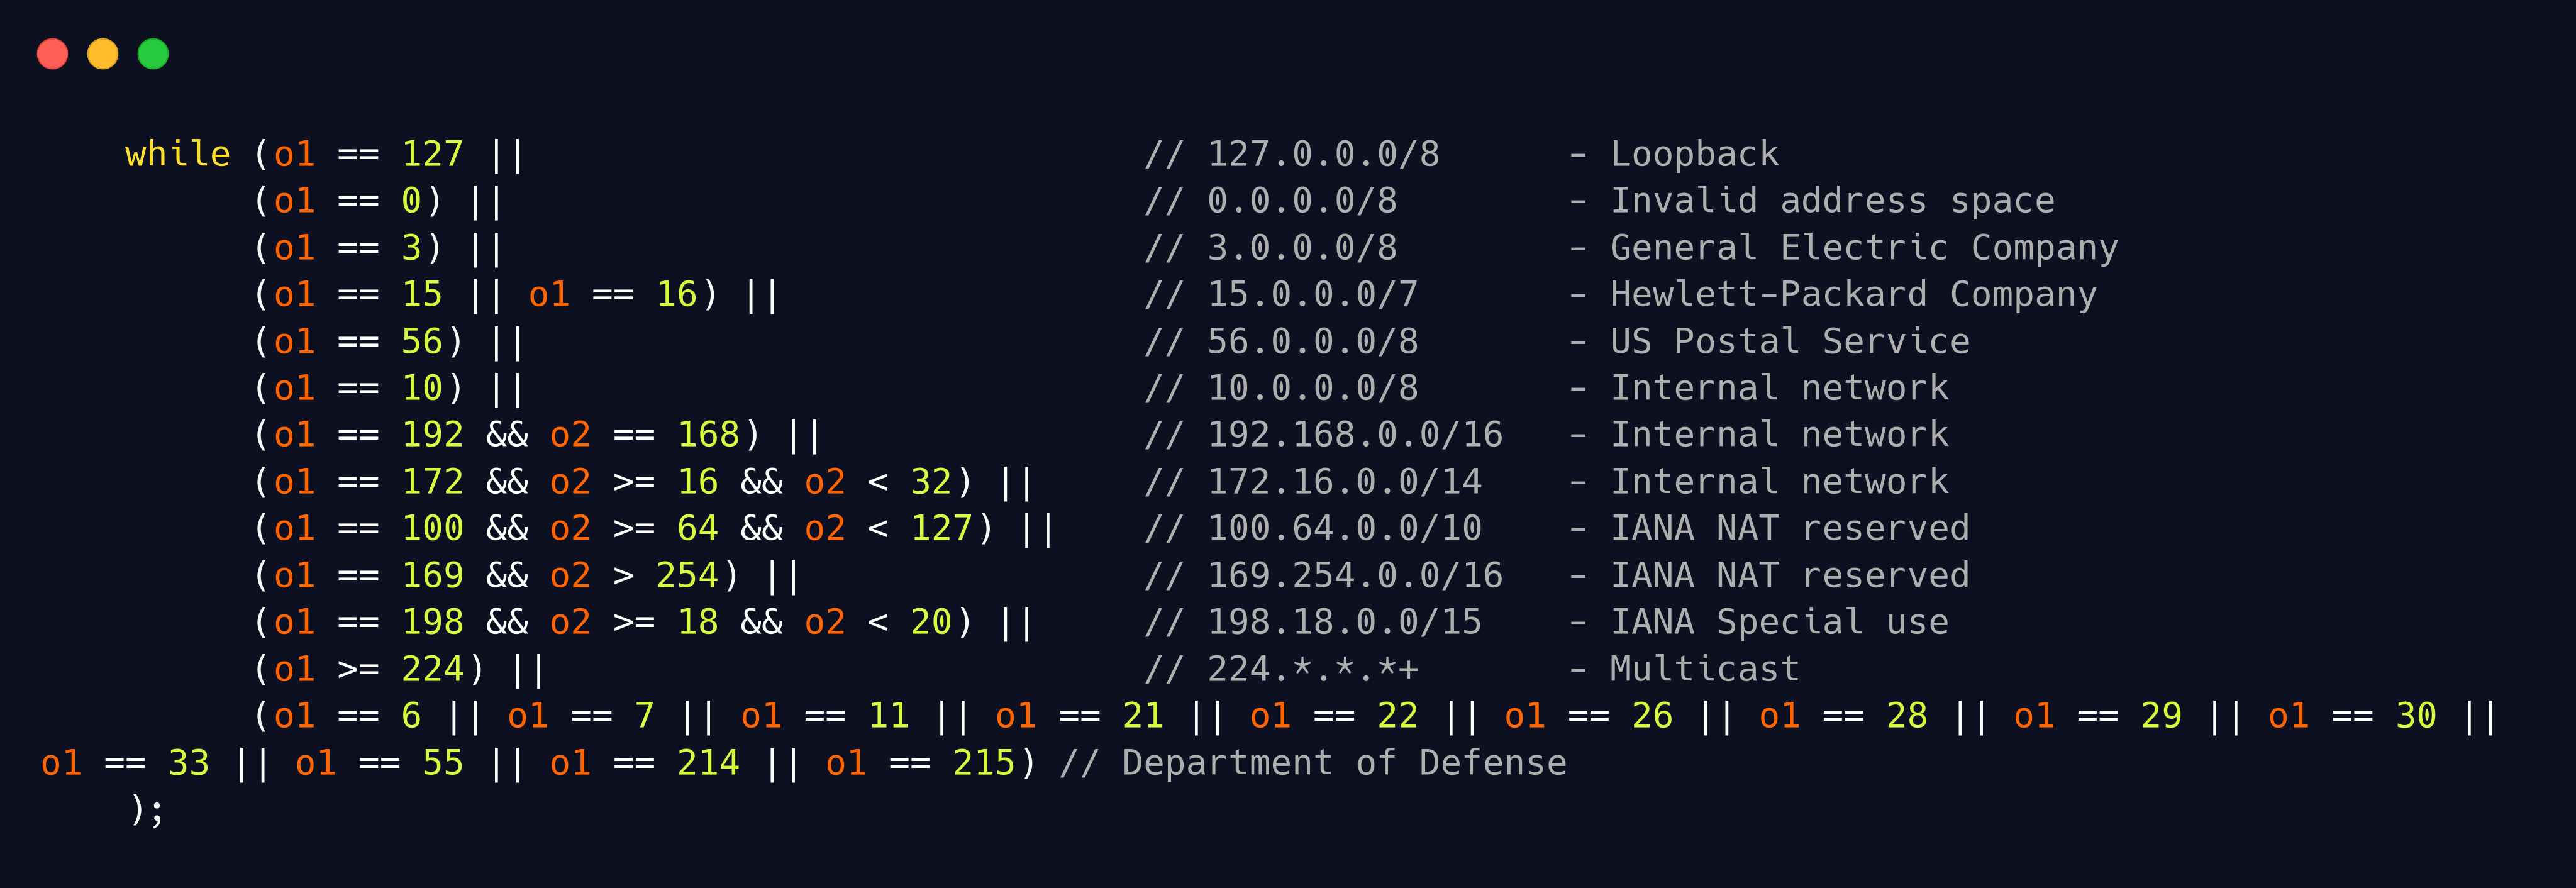
\includegraphics[scale=0.12]{resources/images/get_random_ip.png}
    \caption{Whitelisted IPs in get\_random\_ip function}
    \label{fig:random_ip}
\end{figure}
\section{Mirai Scanner}
The Mirai scanner's source code can be found in the `scanner.c' file. The scanner is used by the bots to search for other devices which are potentially vulnerable to the Mirai malware. The search of the devices is performed using random IP addresses generated using the `get\_random\_ip' function. One interesting aspect of this function is that while being random it skips some IP addresses which are reserved for special purposes, such as the internal addresses or reserved ones. In addition to these addresses there are also some standard IPs which are avoided because, according to the comments in the code, belong to special entities e.g. the `Department of Defense' or the `US Postal Service'. The complete list can be found in Figure~\ref{fig:random_ip}. Instead of performing an entire telnet handshake to check the validity of an IP address the bot sends a TCP SYN packet and if the response it gets is a SYN+ACK packet it starts a dictionary attack against the host. The dictionary is composed of ~60 credentials which are known to be used as default ones (e.g. admin:admin, root:root), all the entries are encrypted to make the reverse engineering harder. More details on the encryption algorithm are provided in Section~\ref{section:ex1}. To handle the possible state transitions of the telnet interaction a switch statement that works as a state machine is used~\cite{de2018ddos}. Once a valid credential is found the bot sends the information to the reporting server which will share it with the loader server. The scanner is also able to detect if the device is already infected by checking if the device is listening on port 48101. If the device is already infected the bot will not try to infect it again~\cite{mirai-hackforum}.
        \chapter{Traffic analysis}
        \chapter{IoT Malware Laboratory}
In order to successfully complete the laboratory activity, it is strongly advised to use the provided virtual machine. The credentials of the root user are `mirai:mirai', this user contains all the necessary information to complete the laboratory. The virtual machine is based on Lubuntu 20.04 LTS, from which unnecessary software has been removed, to make the system lighter and wireshark was installed. The whole lab experience can be performed without giving the machine internet access. \\
The first four exercises have the objective of providing a hands-on experience with the Mirai botnet from the point of view of an attacker who decides to download the source-code and create his own instance.

\section{Mirai botnet initialization}
We decided to use Docker since it provides a lightweight way to create machines that can act both as servers and clients. We also decided to use `docker compose' since it allows us to define and run multi-container Docker applications. To ensure interaction between the containers, we decided to use a custom network to which all the containers are attached. The network is set as `internal' meaning that the containers do not have access to the internet, we used this approach to ensure that the botnet could not attack any real systems. \\
The first step to start the botnet is to start a terminal and run the following commands:
\begin{enumerate}
    \item cd mirai
    \item docker compose up -d
\end{enumerate}
Since the virtual machine comes with all the Docker images pre-built, the services will start almost instantly. The Mirai botnet can be built to work both with telnet and ssh and both in debug and release mode. We opted on using the telnet version, built in debug mode to have unencrypted traffic and to have a better understanding of the botnet's behavior.
This commands will start some docker containers with the following services:
\begin{itemize}
    \item the CNC server (Ubuntu) with the database (MySQL)
    \item 4 containers (Alpine) simulating IoT devices. These four devices are running a telnet server.
    \item a Nginx container to simulate a website (victim)
\end{itemize}
To actually start the botnet, the following command must be executed:
\begin{itemize}
    \item docker exec -it mirai-cnc bash /home/cnc/starter.sh
\end{itemize}
This command will start the CNC server allowing connections from both the bots and the attacker. It is important to notice that the CNC server is running on a fixed IP address which is `192.168.10.10' and that it is possible to access the CNC server from the host machine by using telnet. The CNC server implements a telnet server in GO from which it is possible to interact with the botnet.

\begin{figure}
    \centering
    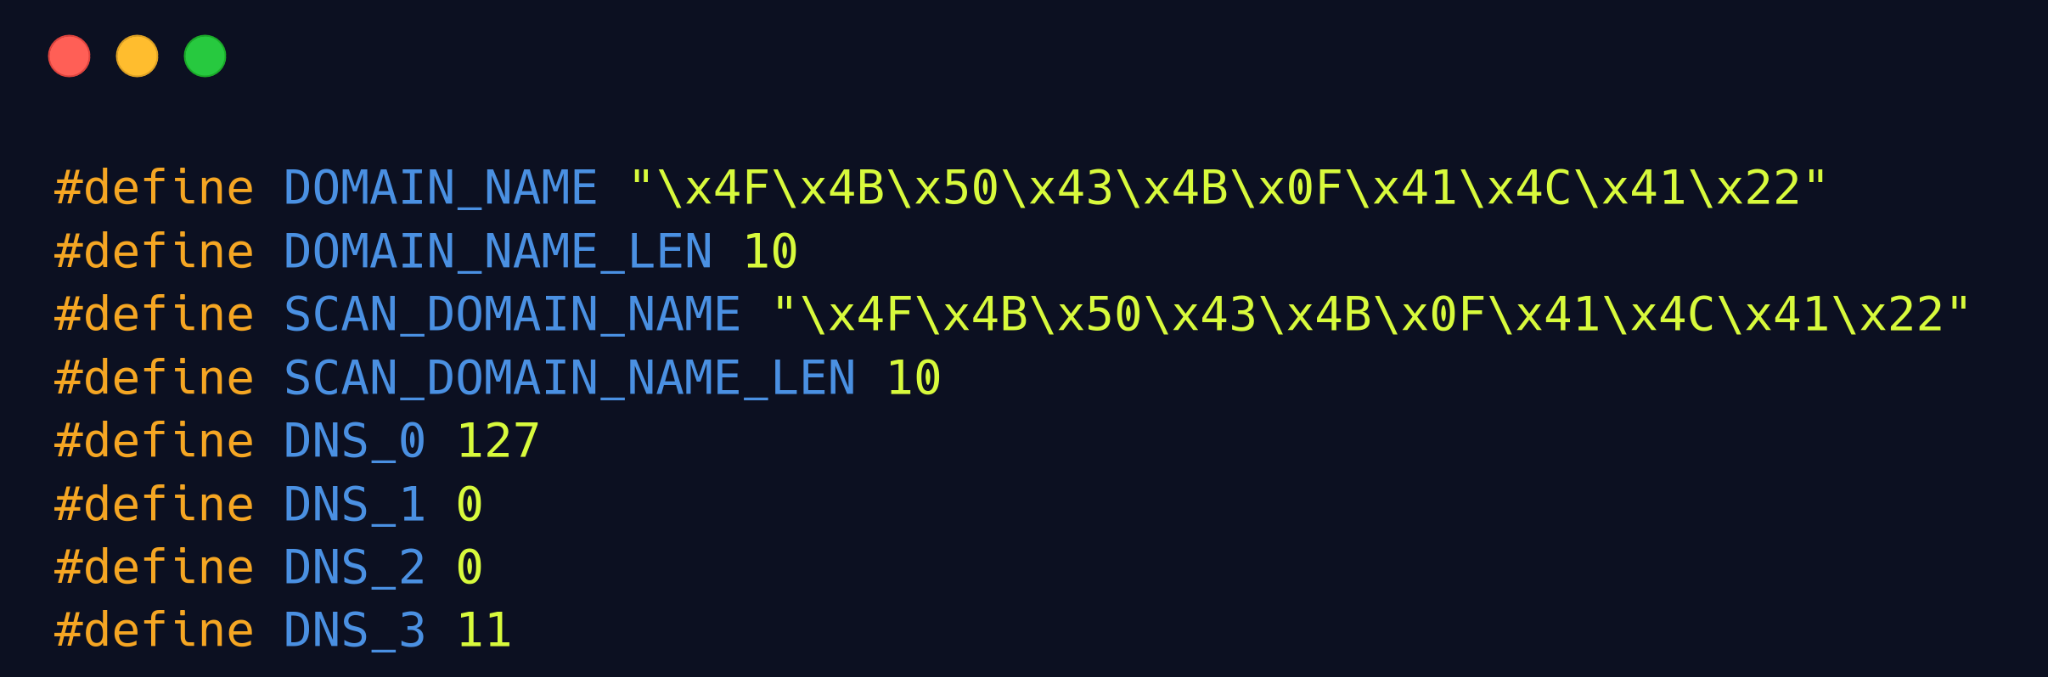
\includegraphics[width=0.8\textwidth]{resources/images/config.png}
    \caption{config.h file}
    \label{fig:config_h}
\end{figure}
\section{Exercise 1: Find the CNC}
\label{section:ex1}
Each bot that is part of the Mirai botnet reports to the CNC its status and waits for commands from it, this means that the bot has to know at any time which how to contact the CNC (IP address and port). To achieve this the bot has the value of a DNS entry which resolves to the CNC IP address hard coded in the binary. The actual entry can be found in the file `bot/config.h' (figure \ref{fig:config_h}) with name `DOMAIN\_NAME'. In the same config file it is possible to find also the `SCAN\_DOMAIN\_NAME' entry which refers to the reporting server to which the bot sends information about the newfound victims, in this case it is the same as the CNC. Together with these entries the bot is also provided with four entries whose name starts with `DNS\_' that are used to indicate the DNS server's address \footnote{In our case the IP is set to 127.0.0.11 which is the address of the Docker internal DNS}. The actual algorithm to encrypt these entries can be found in the file `tools/enc.c', it basically reduces to splitting the key in four parts and using them to XOR each character of the entry. This is probably done to protect the CNC since it would be easy for someone to get the IP address of the CNC by just intercepting the traffic or reversing the binary, and while it is really easy to change an IP address it would be way harder to change the DNS server's address since it is hard coded in the binary.

\section{Exercise 2: Connect to the CNC}
Since the entire infrastructure is run in some containers on the host machine there are two possible ways to connect to the CNC server. The first one employs the usage of the telnet command run from the host machine, `telnet 192.168.10.10' will connect to the CNC server. To check that the CNC IP is actually 192.168.10.10, the command `docker ps' can be run to see the list of running containers and the command `docker container inspect mirai-cnc' can be used to see the container's IP address. The second way to connect to the CNC server is to run the telnet command from the CNC server itself, this can be done by running the command `docker exec -it mirai-cnc telnet localhost'. The credentials of the only existing account are `root:root'. Once inside the CNC server it is possible to use the `?' command to list the possible attacks, and since we are logged in as a privileged user it is possible to use two additional commands `adduser' which adds a user to the CNC server and `botcount' which returns the number of bots connected to the CNC server. The `botcount' command was slightly modified to return the IP addresses of the bots connected to the CNC server together with their number.

\section{Exercise 3: Spread Mirai}
This exercise has the objective of infecting some containers with the Mirai malware, to achieve this the idea is to get access to one of the IoT devices and then use it to infect the other devices. The target device has ip 192.168.10.5. All the IoT devices have the same credentials which are `admin:admin1234', they were originally found in a made up manual page which can be found here TODO: add page. Since the CNC together with the telnet interface provides an endpoint to download files it can be used as the loader server. The first step is to connect to the target machine using the command `telnet 192.168.10.5', after logging in it is possible to get the actual scanner script from the CNC by using the command `wget mirai-cnc/bins/scanner.py'. There are a few things to consider here, the first one is that instead of the IP it is possible to use the container name `mirai-cnc' since we are inside a docker container in the same network. The other important thing to notice is that we decided to reimplement the scanner because the original scanner targets random machines over the internet. The scanner script is written in python and tests a set of credentials against some known IPs. If the scanner is run as-is it would not connect to any device since it is missing the credentials used by the devices. To solve this issue the script must be updated either from the CNC server or from the host machine. If the CNC route is chosen the file can be found in the folder `/var/www/html/bins/', after editing it, downloading it again on the target machine and running it three machines will be infected. It is possible to verify the infected machines from the CNC Telnet interface, by using the `botcount' command. Even though there are four potential victims only three of them will be infected, this is due to a programming error on our side which led to the scanner not targeting the machine with IP `192.168.10.5'.

\begin{figure}
    \centering
    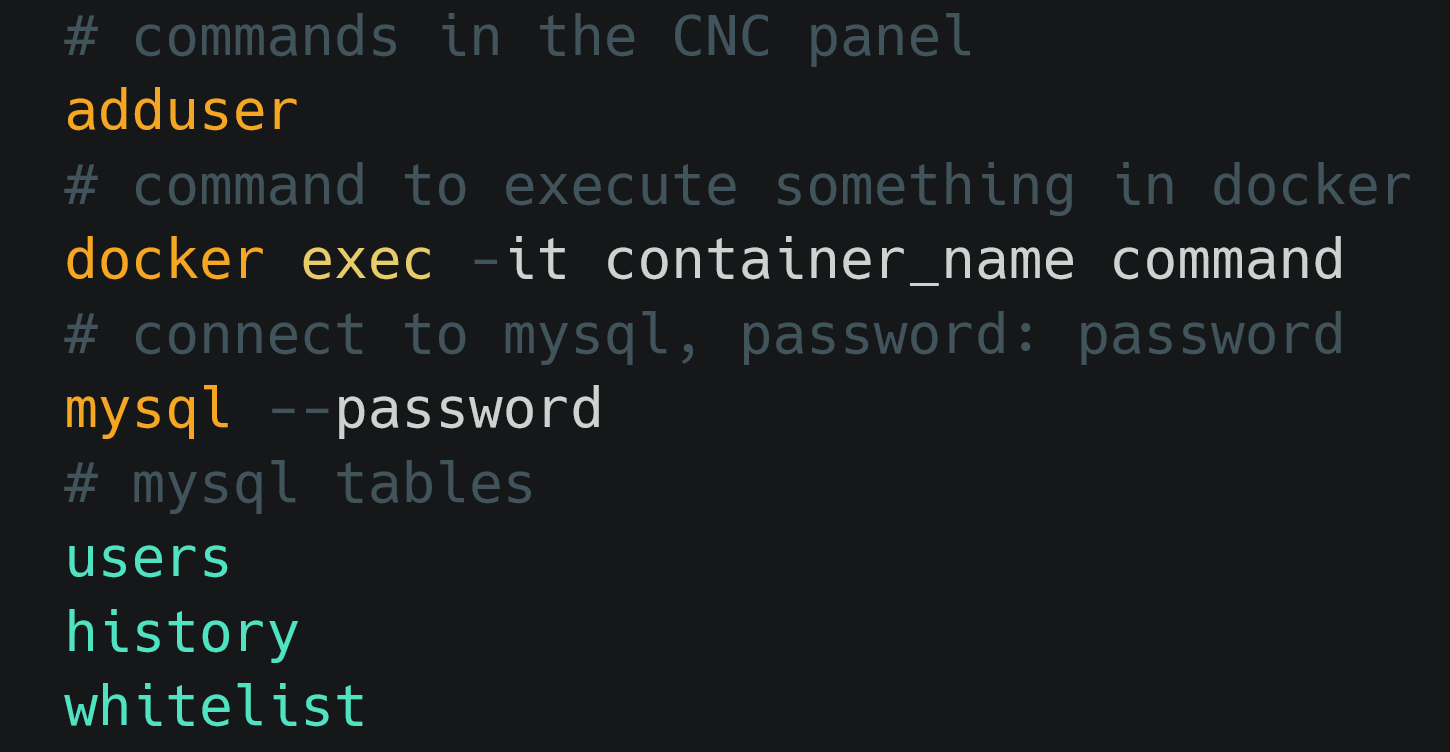
\includegraphics[width=0.8\textwidth]{resources/images/create_user.png}
    \caption{Commands needed for the fourth exercise}
    \label{fig:database}
\end{figure}

\section{Exercise 4: Sell the service}
This optional exercise was created to show how it is possible to create a new user account inside the CNC. All the necessary information to perform this exercise can be found in figure \ref{fig:database}. The first step is to connect to the CNC server using telnet and logging in as the `root' user. By using the `adduser' command the credentials and constraints for the new user can be inserted, an example of this can be found in figure \ref{fig:add_user}. It is important to notice that if no constraint is provided the CNC will not give any error, but the user will not be created. After creating the user it is possible to check the database to check how the user information are stored. The first step to achieve this is to connect to the MySQL database found in the CNC server, this can be done by running the command `docker exec -it mirai-cnc mysql -password', the password is `password'. Once inside the MySQL shell it is possible to run the command `use mirai' to select the database and then `select * from users' to see the table containing the users. The result of this command can be found in figure \ref{fig:table_users}. One interesting thing to notice is that the password is stored in plain text by the original implementation. This is a bad practice and should never be done in a real-world scenario since an attacker compromising the database would have access to the all the accounts. To avoid this issue hashing is used in real-world applications, this way even if the attacker gets access to the database he would not be able to get the actual password. \\
Together with the user accounts the database also stores a list of `whitelisted' IPs which the bots will not attack and a table which contains the log of all the attacks launched by the botnet.

\begin{figure}
    \centering
    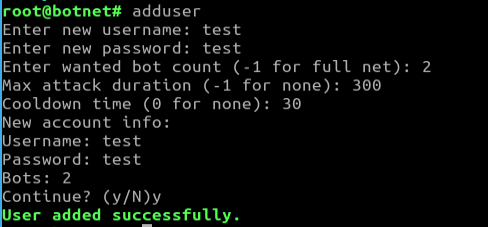
\includegraphics[width=0.8\textwidth]{resources/images/add_user.png}
    \caption{Result of the adduser command}
    \label{fig:add_user}
\end{figure}

\begin{figure}
    \centering
    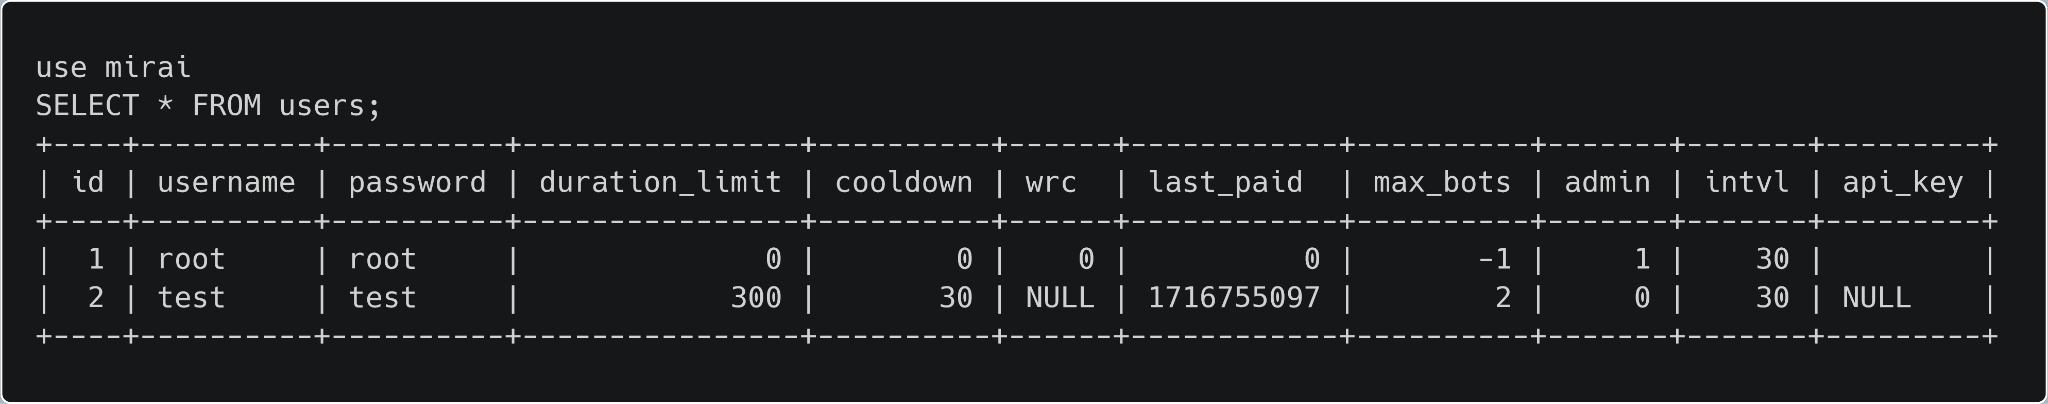
\includegraphics[width=1.0\textwidth]{resources/images/table_users.png}
    \caption{Database content after adding the new user}
    \label{fig:table_users}
\end{figure}
        \chapter{Other malware}

\section{Hajime}

\section{Goldoon}

\section{BotenaGo}

Identified in November 2021 by AT\&T Alien Labs researchers, BotenaGo is a backdoor that provides cybercriminals access to devices through 33 exploit functions. Their first analysis was performed by reverse engineering the malware's binary and it revealed that the malware associates each exploit function with a string that represents a potential target system, similar to a signature. This is needed because the malware sends a ``GET'' request to the target and then searches into the returned data for the signature. For example the string ``\texttt{Server: Boa/0.93.15}'' is mapped to the function \texttt{main\_infectFunctionGponFiber} which exploit the CVE-2020-8958 vulnerability. They also privide a search result on Shodan that shows 2 milion potential targets. This number decreased in the years as you can see in \Cref{fig:boa-shodan}. All the exploits can be found in \Cref{fig:all-vulnerabilities-botenago} which illustrates the \texttt{scannerInitExploit} from its source code.

\begin{figure}[ht]
    \centering
    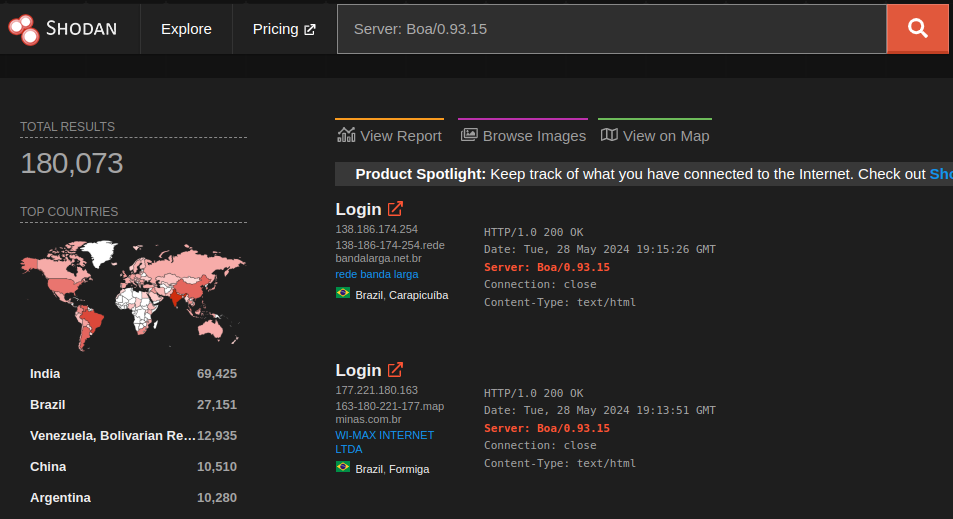
\includegraphics[scale=0.4]{resources/images/boa-shodan.png}
    \caption{Shodan search result for Boa/0.93.15}
    \label{fig:boa-shodan}
\end{figure}

The CNC has two ways of sending command to the infected device:

\begin{enumerate}
    \item Use one of the two backdoor ports (31412 and 19412) to send a command to the device. On port 19412, it lissens for the victim IP address and once received it tries each exploit on that IP.
    \item It listens on a system IO user input. For example it can be accessed locally by using telnet. 
\end{enumerate}

In 2022 its source code was leaked on GitHub and AT\&T Alien Labs provided another analysis which did not provide new information but confirmed the previous analysis. \cite{att-botenago-reverse,att-botenago-sourcecode}

\begin{figure}[ht]
    \centering
    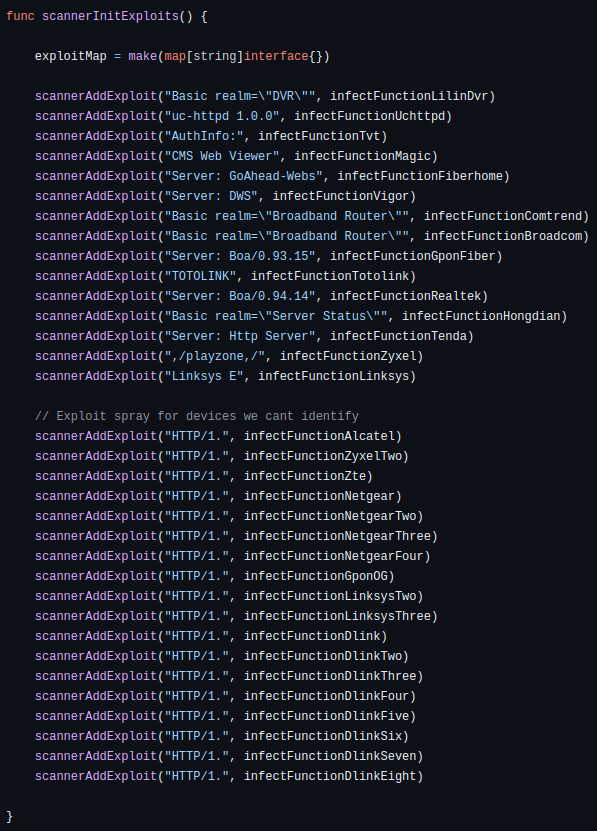
\includegraphics[scale=0.5]{resources/images/all-vulnerabilities-botenago.png}
    \caption{All the vulnerabilities exploited by BotenaGo}
    \label{fig:all-vulnerabilities-botenago}
\end{figure}

\section{Malware comparison}


        \chapter{Conclusion}

    \endgroup

    \addcontentsline{toc}{chapter}{Bibliography}
    \bibliographystyle{plain}
    \bibliography{biblio}
    
    \titleformat{\chapter}{\normalfont\Huge\bfseries}{Allegato \thechapter}{1em}{}    
\end{document}
